\chapter{A Megoldó használata}
\thispagestyle{empty}

A Calc \textbf{Eszközök} menüpontjában található a
\textbf{Megoldó} (angolul Solver). Segítségével megkereshetjük egyenleteket, egyenlőtlenségeket kielégítő változók azon értékeit,
amelyek a \textbf{célcellában} optimális eredményt adnak. Megadhatjuk, hogy a célcellában az érték maximális, minimális, vagy egy adott értéket megközelítő legyen. Meghatározhatunk több
 korlátozó feltételt is az egyes cellákra.

A következő feladat a Megoldó használatára mutat példát.


\section{35. feladat}

{\itshape
Egy bútorkészítő üzemben
négyféle konyhabútor készítenek. Ezeket ,,My way'', ,,Lacelli'',
,,Pulsar'' és ,,Orfix'' néven hozzák forgalomba. A
bútorgyártás költségeit öt részre osztották: ,,Munkafelvétel'',
,,Látványterv készítés'', ,,Anyagár és asztalosmunka'',
,,Szállítás és összeszerelés'' és ,,Egyéb'', előre nem látható
kiadások. Az egyes konyhabútorok esetén a költségeket
(Euroban) \aref{Költségek} táblázat mutatja.}

\begin{table}[!h]
\begin{center}
\caption{Konyhabútorok költségei}\label{Költségek}
\begin{tabular}{|c|c|c|c|c|c|}
\hline
 & \multicolumn{5}{c|}{Költségek}\\ \cline{2-6}
Konyhabútorok & Munkafelvétel & Látványterv & Anyagár és &
Szállítás és & Egyéb\\ 
 & & készítés & asztalosmunka & összeszerelés & \\ \hline
My way & 150 & 200 & 800 & 200 & 250\\ \hline
Lacelli & 100 & 500 & 1200 & 250 & 200\\ \hline
Pulsar & 100 & 150 & 1000 & 400 & 300\\ \hline
Orfix & 150 & 200 & 1100 & 300 & 200\\ \hline
\end{tabular}
\end{center}
\end{table}

{\itshape
A vállalatnak az egyes termékeken
darabonként rendre 550, 700, 500 és 650
Euro haszna van. Egy adott időszakban az
egyes tevékenységekre elkölthető összegek korlátozottak.
,,Munkafelvétel''-re 10~000, ,,Látványterv készítés''-re 20~000,
,,Anyagár és asztalosmunkára'' 70~000, ,,Szállítás és
összeszerelés''-re 40~000 és ,,Egyéb'' kiadásokra legfeljebb 30~000
Euro költhető. }

{\itshape
További korlátozó feltételek még, hogy a ,,Szállítás és
összeszerelés'' költsége legfeljebb negyede lehet az ,,Anyagár és
asztalosmunka'' költségeinek, valamint ,,Pulsar''-ból legalább 5-öt
mindenképpen gyártani kell.}

{\itshape
Mennyit gyártson a vállalat az egyes termékekből a vizsgált
időszakban, hogy a haszna maximális legyen?}

\clearpage
A feladat megoldása, az alábbi lineáris programozási feladat
megoldását jelenti:

Feltételek:
\begin{eqnarray*}
150x_1+100x_2+100x_3+150x_4&\leqslant &10000\\
200x_1+500x_2+150x_3+200x_4&\leqslant &20000\\
800x_1+1200x_2+1000x_3+1100x_4&\leqslant &70000\\
200x_1+250x_2+400x_3+300x_4&\leqslant &40000\\
250x_1+200x_2+300x_3+200x_4&\leqslant &30000\\
200x_1+250x_2+400x_3+300x_4&\leqslant
&0,25(800x_1+1200x_2+1000x_3+1100x_4)\\
x_{3}&\geqslant &5
\end{eqnarray*}
\begin{center}
$x_{1},x_{2},x_{3},x_{4}$ nem negatív egészek
\end{center}

Célfüggvény, amit most maximalizálni kell:
$550x_{1}+700x_{2}+500x_{3}+650x_{4}$

Hozzuk létre az alábbi táblázatot egy új munkalapon (\ref{35-feladat}
ábra).

\begin{figure}[!h]
\begin{center}
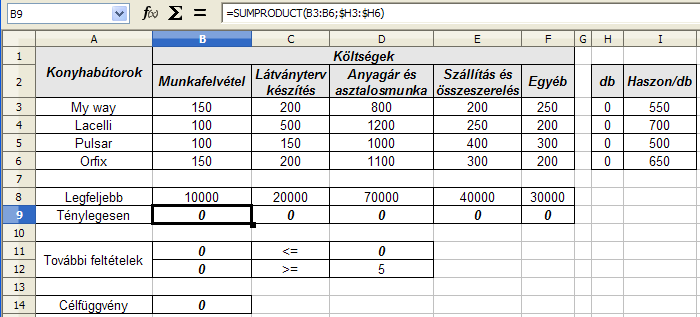
\includegraphics[width=15.999cm]{oocalcv1-img170.png}
\caption{35. feladat}\label{35-feladat}
\end{center}
\end{figure}

A C9:F9 tartományt \aref{35-feladat} ábrán látható tartalmú B9 cella
\textsf{(=SUMPRODUCT(B3:B6;\$H3:\$H6))} másolásával hozzuk létre.
Ebben a sorban tényleges
költségrészletek fognak megjelenni a Megoldó által
meghatározott darabszámok (H3:H6) és a részköltség
összegek alapján. A további képlettel feltöltött cellákat
\aref{Feltöltés} táblázat mutatja.

\begin{table}[!h]
\begin{center}
\caption{A cellák tartalma}\label{Feltöltés}
\begin{tabular}{|c|l|}
\hline
\textbf{Cellacím}&
\multicolumn{1}{|c|}{\textbf{Cellatartalom}}\\ \hline
B11 & \sffamily =E9\\ \hline
B12 & \sffamily =H5\\ \hline
D11 & \sffamily =D9*0,25\\ \hline
B14 & \sffamily =SUMPRODUCT(H3:H6;I3:I6)\\ \hline
\end{tabular}
\end{center}
\end{table}

A \textbf{Megoldó} ablakában válasszuk \textbf{Célcellának} a
B14-et, a H3:H6 cellák módosításával. Válasszuk a
\textbf{Maximalizál} kapcsolót. Minden feltételt vegyünk fel
egyesével a \textbf{Hozzáadás} kapcsolóra kattintva (\ref{35-feladat2}
ábra).

Kizárólag egész értékeket engedélyezünk, ezt a kapcsolót
a \textbf{Beállítások} gombra kattintva érjük el.

\begin{figure}[!h]
\begin{center}
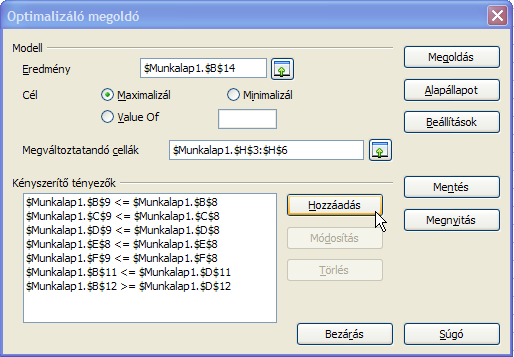
\includegraphics[width=12.598cm]{oocalcv1-img171.png}
\caption{35. feladat}\label{35-feladat2}
\end{center}
\end{figure}

Kattintsunk a \textbf{Megoldás} feliratú gombra. A megjelenő
ablak értesít minket, hogy sikerült megoldást találni. A
H3:H6 tartományban megjelentek azok a darabszámok, amelyeknél a
feltételeknek megfelelve, a legnagyobb nyeresége lesz az üzemnek
(\ref{35-feladatMegoldás} ábra).

\begin{figure}[!h]
\begin{center}
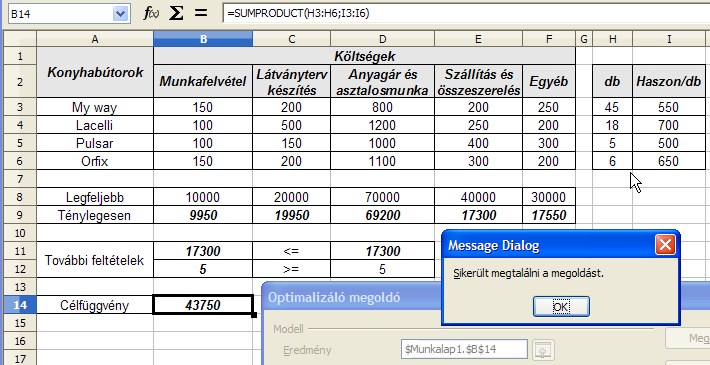
\includegraphics[width=14.999cm]{oocalcv1-img172.png}
\caption{35. feladat --  Megoldás}\label{35-feladatMegoldás}
\end{center}
\end{figure}

